%!Mode:: "TeX:UTF-8"
%!TEX encoding = UTF-8 Unicode
%!TEX TS-program = xelatex
\documentclass{ctexart}
\usepackage{float}
\newif\ifpreface
%\prefacetrue
\input{../../../global/all}
\begin{document}
\large
\setlength{\baselineskip}{1.2em}
\ifpreface
  \input{../../../global/preface}
  \newgeometry{left=2cm,right=2cm,top=2cm,bottom=2cm}
\else
  \newgeometry{left=2cm,right=2cm,top=2cm,bottom=2cm}
  \maketitle \fi
%from_here_to_type
\begin{problem}\label{pro:1}
  Assume \(A=\{a \in P \mid a \mid m\} = \{q_i \mid i=1,\cdots,s\}\), where \(P \subset \mathbb{N}\), \(\forall p \in P\), \(p\) is prime,
  \(s = |A|\).
  Prove: \(g\) is the primative root mod \(m\) \(\iff\)
  \(g\) is \(q_i\)-tic non-residue mod \(m\), \(\forall i=1,\cdots,s\).
\end{problem}
\begin{solution}
  On one hand, assume \(g\) is \(q_i\)-th power residue of \(m\), then \(g \equiv h^{q_i} \mod m\).
  So \(g^{\frac{\phi(m)}{q_i}}\equiv h^{\phi(m)}\equiv 1 \mod m\), contradiction!

  On the other hand, assume \(o(g)<\phi(m)\). Easily \(o(g) \mid \phi(m)\), so \(\frac{\phi(m)}{o(g)} \in \mathbb{Z}\).
  So \(\exists i,q_i \mid \frac{\phi(m)}{o(g)}\). Then \(g^{\frac{\phi(m)}{q_i}} \equiv 1 \mod m\).
  Then \(g\) is \(q_i\)-th power residue of \(m\).
\end{solution}

\begin{problem}\label{pro:2}
  Prove:
  \begin{enumerate}
    \item \(10\) is the primative root mod \(17,257\).
    \item The length of repetend of \(\frac{1}{17}\) is \(16\), the length of repetend of \(\frac{1}{257}\) is \(256\).
  \end{enumerate}
\end{problem}
\begin{solution}
  Easily \(\phi(17)=16=2^4\). So we only need to check \(10^8 \not \equiv 1 \mod 17\).
  Easily \(10^8 \equiv 100^4 \equiv (-2)^4 \equiv 2^4 \equiv -1 \mod 17\).
  So \(10\) is primative root of \(17\).

  Easily \(\phi(257)=256=2^8\), so we only need to check \(10^{128} \not \equiv 1 \mod 257\).
  By calculation easily to get that \(10^{128}\equiv -1 \mod 257\).
  So \(10\) is primative root of \(17\).

  Since \(10\) is primative root of \(17,257\), we know the length of loop-body of \(\frac{1}{17},\frac{1}{257}\) are \(16,256\).
\end{solution}

\begin{problem}\label{pro:3}
  Apply index table to solve the equation \[
    x^{15 } \equiv 14 \pmod{41}.
  \]
\end{problem}
\begin{solution}
  Use \(6\) as primative root of \(41\), we have this table of index:
  \begin{figure}[H]
    \centering
    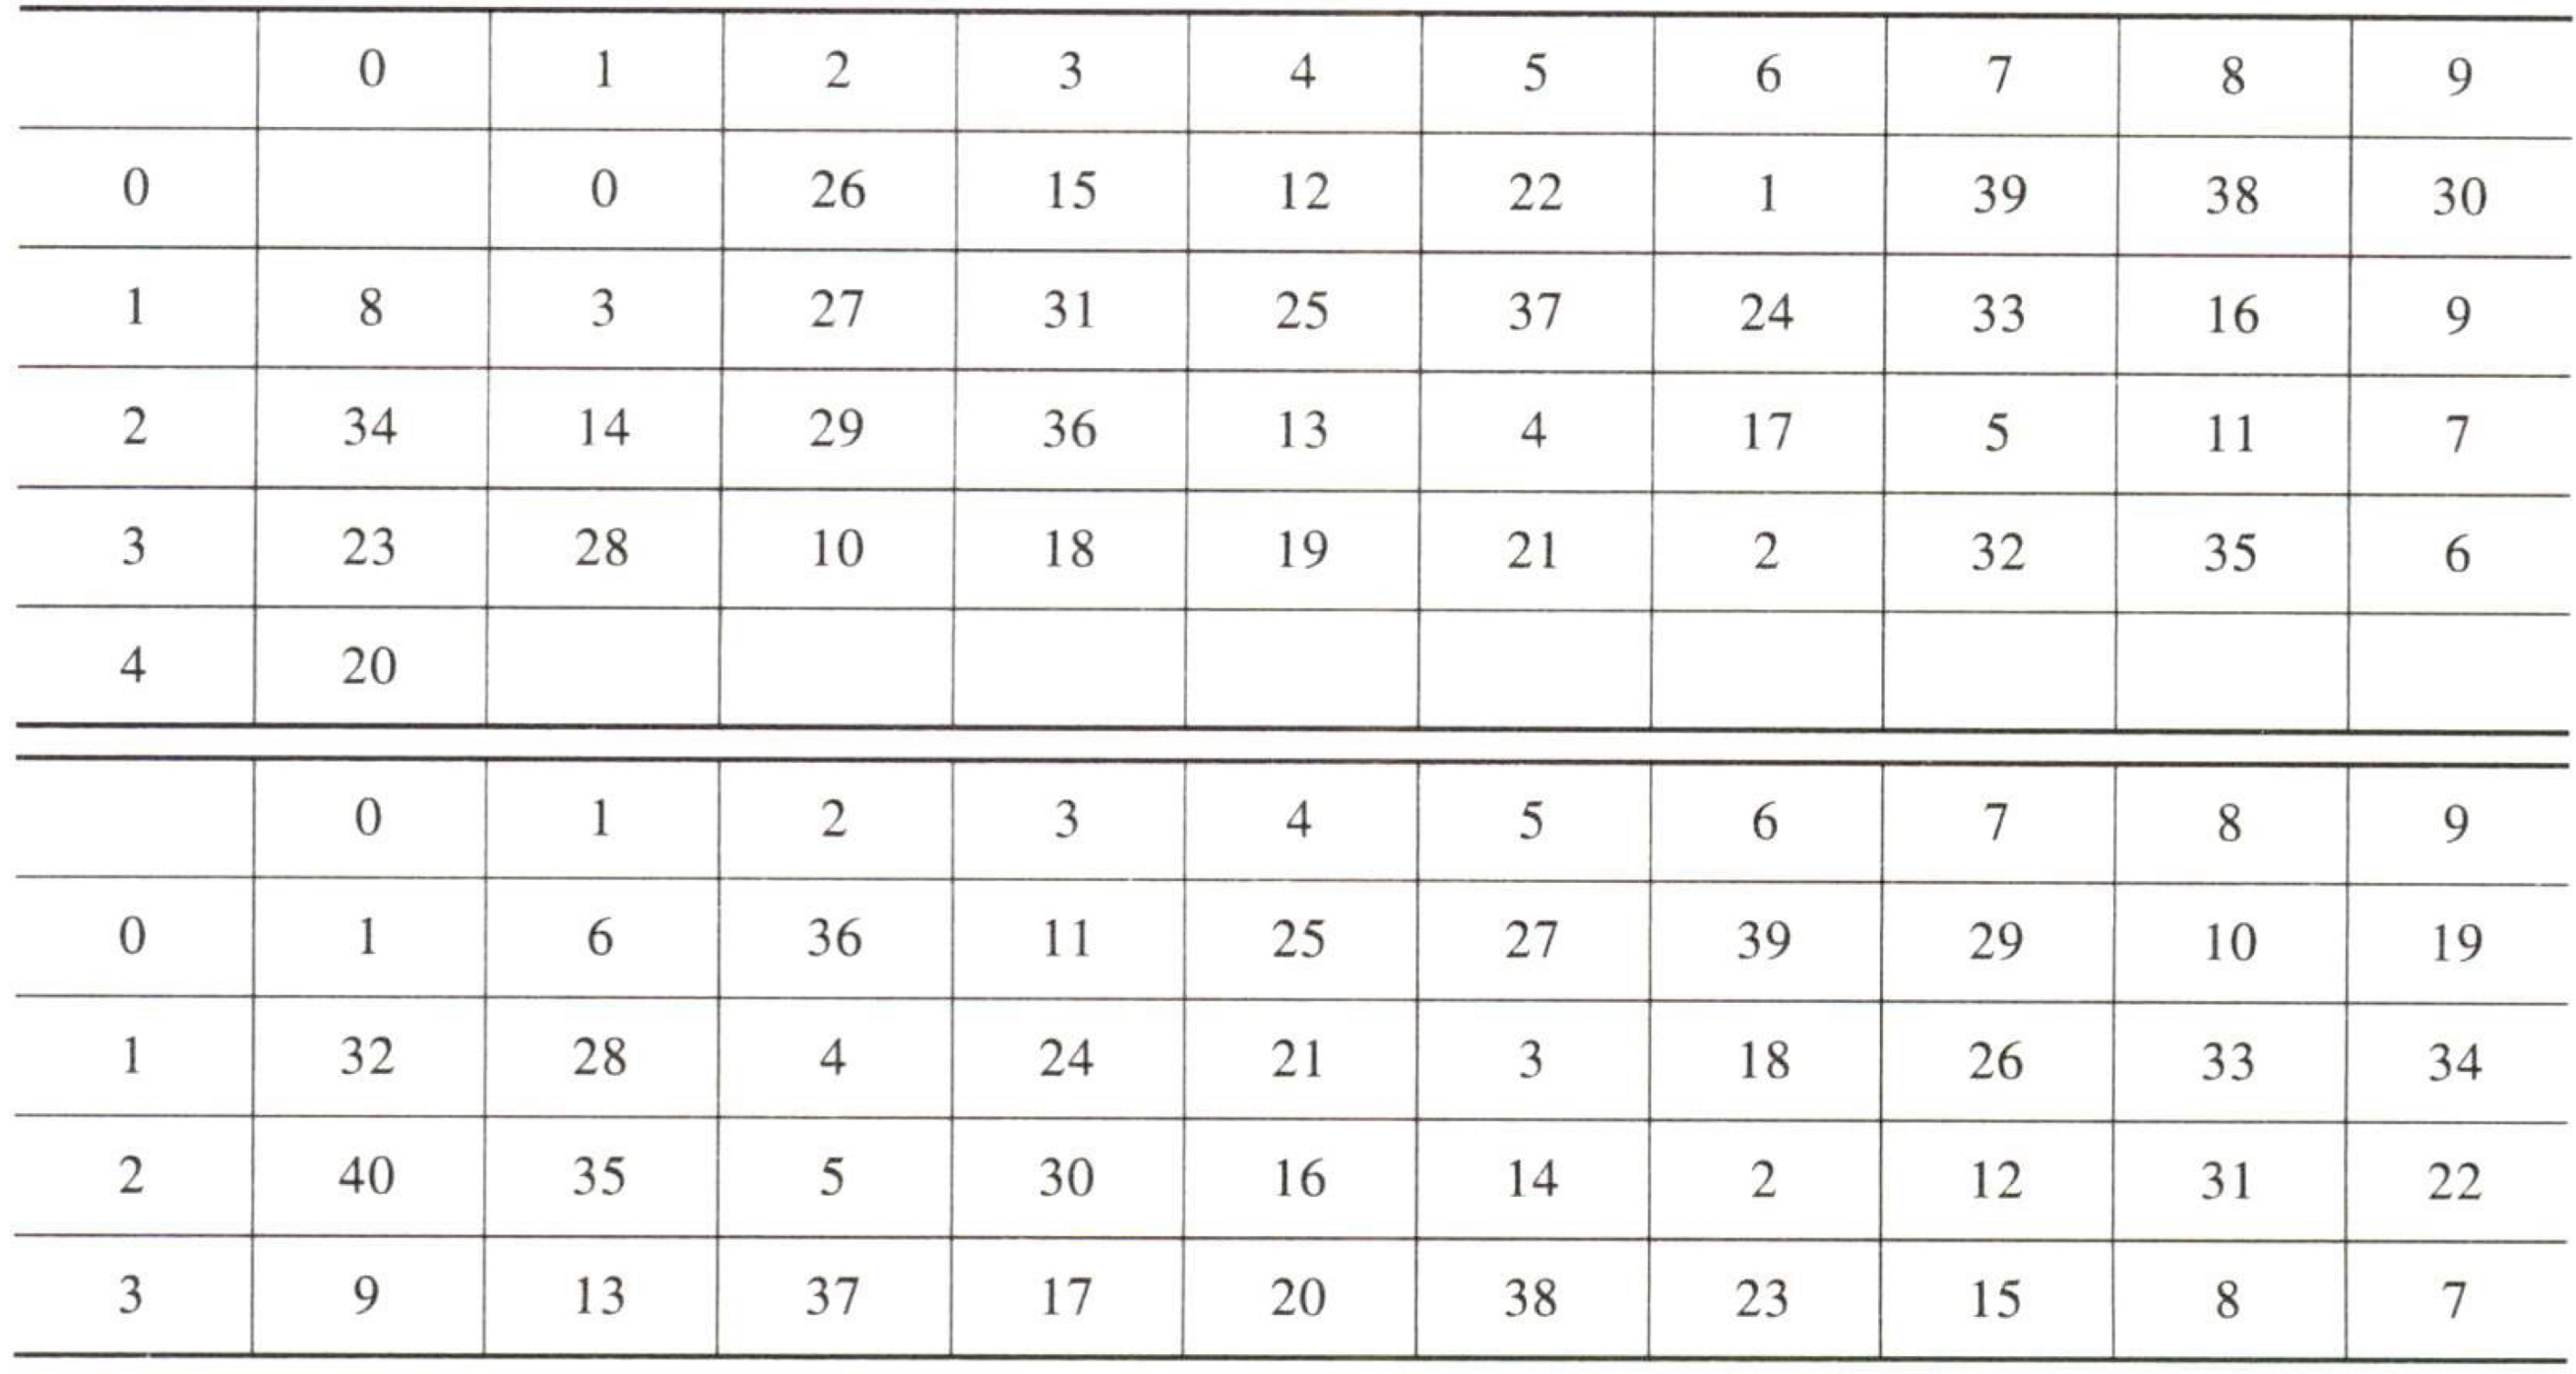
\includegraphics[width=\linewidth]{./mod41.png}
  \end{figure}
  Then \(x^{15} \equiv 14 \mod 41 \iff 15 \ind x \equiv \ind 14 \mod 40 \iff 3 \ind x \equiv 5 \mod 8 \iff \ind x \equiv 7 \mod 8\).
  So \(\ind x = 7,15,22,29,36\). So \(x \equiv 29,3,5,22,23 \mod 41\).
\end{solution}

\begin{problem}\label{pro:4}
  Assume \(m >2\) has primative root, prove \(\forall g\) is the primative root mod \(m\),
  \(\ind_g -1=\frac{1}{2}\phi(m)\).
\end{problem}
\begin{solution}
  We have \(g^{\phi(m)} \equiv 1 \mod m\).
  So \(\ind_g 1=0\).
  Since \((-1)^2 \equiv 1 \mod m\), we have \(2 \ind_g -1 \equiv \ind_g 1 \mod \phi(m)\).
  So \(\ind_g -1 \equiv 0 \mod \frac{\phi(m)}{2}\).
  But obviously \(\ind_g -1 \neq 0\), so we obtain \(\ind_g -1 = \frac{\phi(m)}{2}\).
\end{solution}

\begin{problem}\label{pro:5}
  Assume \(g_1,g_2\) are two primative root mod \(m\), prove:
  \begin{enumerate}
    \item \(\ind_{g_1}g \cdot \ind_{g}g_1 \equiv 1 \pmod{\phi(m)}\);
    \item \(\ind_g a \equiv \ind_g g_1 \cdot\ind_{g_1}a \pmod{\phi(m)}\)
  \end{enumerate}
\end{problem}
\begin{solution}
  \begin{enumerate}
    \item Let \(a=\ind_{g_1}g,b=\ind_{g}g_1\).
      By the defination, we can get that \(g_1^a \equiv g \pmod{\phi(m)}, g^b \equiv g_1 \pmod{\phi(m)}\).
      Then \((g_1^{a})^b = g_1^{ab}\equiv g^b \equiv g_1 \pmod{\phi(m)}\).
      Since \(g_1\) is the primative root of \(m\), then \(ab \equiv 1 \pmod{\phi(m)}\).
    \item Only need to check \(g^{\ind_g g_1 \cdot \ind_{g_1} a} \equiv a \mod m\).
      Easily \(g^{\ind_g g_1 \cdot \ind_{g_1} a} \equiv g_1^{\ind_{g_1} a}\equiv a \mod m \).
  \end{enumerate}
\end{solution}

\end{document}
